\section{Theoretical Background}
\label{sec:Theory}

In this section the theoretical background that is necessary for this experiment is being discussed.

\subsection{Interaction of photons with matter}

Photons interact with matter in a probabilistic way, that is dependend on the energy of the photon and the type of matter it interacts with.
The interaction mechanisms themselves can in principle be broken down into three different types of interaction, namely the photo-effect, compton-effect and pair-production. \\

What exactly happens in these processes is described later on. 
From a theoretical perspective the probabilities for the given mechanism can be described via cross-sections $\sigma$. 
The energy-dependence of these cross-sections is being shown in~\autoref{fig:exctinct} where the extinction coefficient $\mu = n \sigma$, whith the particle density $n$ is being plotted.
This extinction coefficient $\mu$ is primarily relevant when looking at the probability $P$ of a photon being scattered at distance $z$ when going through matter, which is 
\begin{align}
    P(z) = 1 - \exp(-\mu z) \, .
\end{align}

\begin{figure}[htbp]
    \centering
    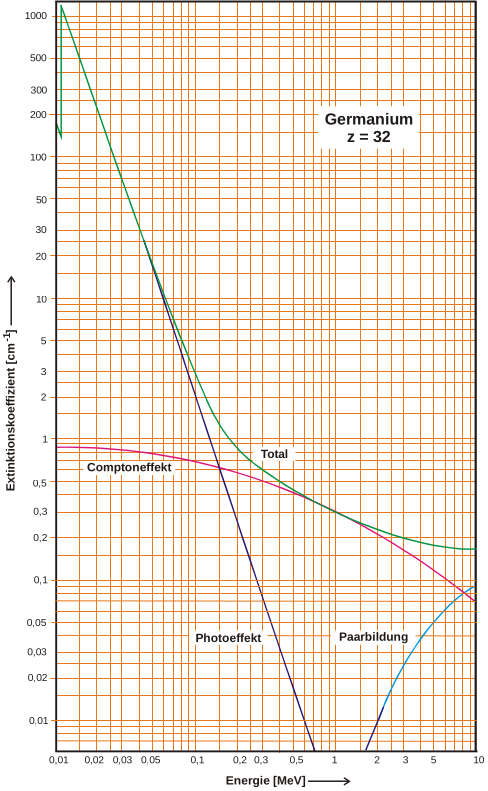
\includegraphics[height=\textwidth]{content/pics/extinct2.png}
    \caption{Partial extinction coefficients in dependence of energy for germanium~\cite{gamma-absorb}.}
    \label{fig:exctinct}
\end{figure}

\textbf{Photo effect} \\

The photo effect describes the phenomenon, when a photon is being absorbed by a shell electron of an atom, where the electron leaves the atom with a kinetic energy of $E_\T{kin} = E_\gamma - E_\T{ion}$, where $E_\gamma$ and $E_\T{ion}$ are the photonenergy and energy needed to ionize the atom.
This effect can only occur for bound electrons, as the momentum is only conserved, when the nucleus absorbs the knockback of the photon. \\
For $\gamma$-photons it is true, that their energy is so high, that the electrons that absorb their energy ionize many more secondary electrons in the solid each.
This has the effect, that the number of created quasifree electrons (and positive holes) in the solid is proportional to the photon energy. \\

\textbf{Compton effect} \\

For higher photon energies the compton effect gets more relevant. 
The compton effect descibes the inelastic scattering of photons with electrons, as seen in~\autoref{fig:compton}.

\begin{figure}[htbp]
    \centering
    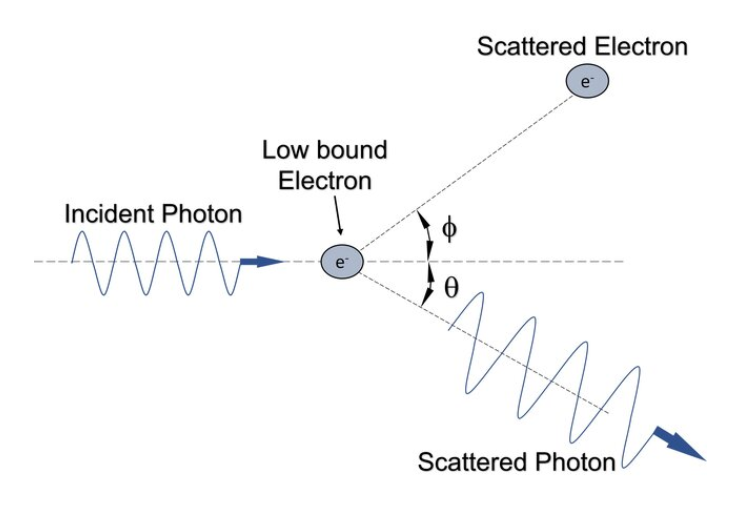
\includegraphics[width=0.7\textwidth]{content/pics/compton.png}
    \caption{Scheme of compton scattering~\cite{traczRFLINACDESIGN2022}.}
    \label{fig:compton}
\end{figure}

The final energy $E_\gamma'$ of the incident photon can be calculated via 
\begin{align}
    E_\gamma' &= \frac{E_\gamma}{1 + \frac{E_\gamma}{m_e c^2} (1 - \cos(\Theta))} \, ,
\end{align}
with scattering angle $\Theta$ and incident photon energy $E_\gamma$.
For an angle of $\Theta = 180^{\circ}$, the maximal possible energy gets transfered to the electron, which then can be oberserved in the detector as the compton edge.

For the differential corss section of the compton effect, the Klein-Nishina-formula~\cite{sandnerQuantenelektrodynamikEinfuehrungFuer2023}
\begin{align}
    \dif{\sigma}{\cos(\Theta_\T{Lab})} = \frac{e^4}{16\pi m^2} \left(\frac{E_\gamma'}{E_\gamma}\right)^2 \left(\frac{E_\gamma}{E_\gamma'} + \frac{E_\gamma'}{E_\gamma} - \sin^2(\Theta_\T{Lab})\right)
\end{align}
can be used. \\

\textbf{Pair production} \\

When the photon energy is above $2m_e c^2 \approx \qty{1.022}{MeV}$, then the incident photon can create an electron-positron-pair, in the vicinity of a nucleus for it to absorb the recoil. 
As the photon energies relevant for this experiment are not above this threshold, this effect does play no role here and is just mentioned for completeness.


\subsection{Detection using germanium detectors}

A germanium detector uses the semiconducting properties of the main material, namely a germanium crystal. 
Germanium is an indirect semiconductor with a small band gap of $\Delta = \qty{0.67}{eV}$~\cite{bandstructurege}, which is why it has to be cooled with liquid nitrogen, in order for it to not have too much noise due to excited thermal electrons.



- germanium band structure (vllt pic einfügen)  
 -> why is it good for detecting? (what about the indirect band gap)

- pn junction stuff
    -> depletion zone with reverse bias(paar grafiken aus diesem buch übernehmen, erklären)

- was passiert mit charge collection und pre-amp?











% \subsection{Properties of monochromatic gamma-emitters in germanium detectors}




% \subsection{Error Calculation}
% % Error Calculation
% The error calculation in this protocoll is being done using the gaussian error propagation
% \begin{equation}
%     \sigma_f = \sqrt{\left( \frac{\partial f}{\partial x_1} \sigma_{x_1} \right)^2 + \left( \frac{\partial f}{\partial x_2} \sigma_{x_2} \right)^2 + ...} \, ,
% \end{equation}
% as well as the formulas 
% \begin{equation}
%     \overline{x} = \frac{1}{n} \sum^n_{i=1}x_i \, ,
%     \label{eq:mittelwert}
% \end{equation}
% for the mean and 
% \begin{equation}
%     \sigma_{\overline{x}} = \frac{\sigma_x}{\sqrt{n}} = \sqrt{\frac{1}{n(n-1)}  \sum^n_{i=1} \left( x_i - \overline{x}\right)^2 } \, ,
%     \label{eq:abweichung}
% \end{equation}
% for the standard deviation. 
% To simplify these calculations, the Python-package \textit{uncertainties}~\cite{uncertainties} is being used. 

\clearpage